\section{Results}

\subsection{Quantitative Evaluation}

% Cross-dataset performance table
\begin{table}[H]
\centering
\caption{Cross-Dataset Performance Evaluation on Validation Sets}
\label{tab:cross_dataset_results}
\begin{tabular}{@{}lccccc@{}}
\toprule
\textbf{Dataset} & \textbf{IoU@0.5} & \textbf{IoU@0.7} & \textbf{IoU@0.9} & \textbf{mIoU} & \textbf{oIoU} \\
\midrule
AERIAL-D & -- & -- & -- & -- & -- \\
RefSegRS & -- & -- & -- & -- & -- \\
RRSIS-D & -- & -- & -- & -- & -- \\
NWPU-Refer & -- & -- & -- & -- & -- \\
\bottomrule
\end{tabular}
\end{table}

% Dataset comparison table
\begin{table}[H]
\centering
\caption{Comparison with Existing RRSIS Datasets}
\label{tab:dataset_comparison}
\resizebox{\textwidth}{!}{%
\begin{tabular}{@{}lccccccr@{}}
\toprule
\textbf{Dataset} & \textbf{Image Resolution} & \textbf{Images} & \textbf{Annotations} & \textbf{Single-object} & \textbf{Multi-object} & \textbf{Resolution} & \textbf{Annotation Generation} \\
\midrule
RefSegRS & 0.13m & 4420 & 4420 & \checkmark & $\times$ & 512 & Manual \\
RRSIS-D & 0.5m-30m & 17402 & 17402 & \checkmark & $\times$ & 800 & Semi-auto \\
NWPU-Refer & 0.12m-0.5m & 15003 & 49745 & \checkmark & \checkmark & 1024-2048 & Manual \\
\midrule
\textbf{AERIAL-D} & \textbf{0.3m-2m} & \textbf{43,514} & \textbf{1,545,994} & \textbf{\checkmark} & \textbf{\checkmark} & \textbf{480} & \textbf{Automated + LLM} \\
\bottomrule
\end{tabular}%
}
\end{table}

\subsection{Qualitative Analysis}

% Qualitative examples figure
\begin{figure}[H]
\centering
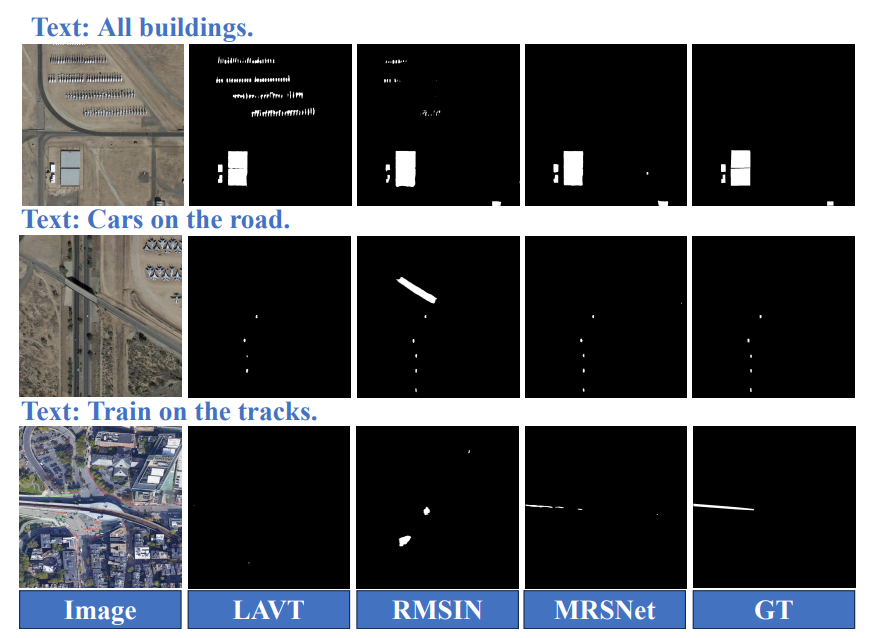
\includegraphics[width=\textwidth]{qualitative.png}
\caption{Qualitative segmentation results from RSRefSeg model on AERIAL-D validation set.}
\label{fig:qualitative_examples}
\end{figure}

% Dataset errors figure
\begin{figure}[H]
\centering
% \includegraphics[width=\textwidth]{errors.png}
\caption{Dataset error analysis examples for LLM-generated unique expressions.}
\label{fig:dataset_errors}
\end{figure}

\subsection{Ablation Studies}

% Ablation expression types table
\begin{table}[H]
\centering
\caption{Ablation Study: Expression Type Training Analysis}
\label{tab:ablation_expression_types}
\resizebox{\textwidth}{!}{%
\begin{tabular}{@{}lcccccc@{}}
\toprule
\textbf{Training Configuration} & \textbf{IoU@0.5} & \textbf{IoU@0.7} & \textbf{IoU@0.9} & \textbf{mIoU} & \textbf{oIoU} & \textbf{Training Expressions} \\
\midrule
Rule-based Only & -- & -- & -- & -- & -- & -- \\
Language Variations & -- & -- & -- & -- & -- & -- \\
Unique Expressions & -- & -- & -- & -- & -- & -- \\
Combined All & -- & -- & -- & -- & -- & -- \\
\bottomrule
\end{tabular}%
}
\end{table}


